\documentclass[11pt]{article}
\usepackage[utf8]{inputenc}
\usepackage[dvips]{graphicx}
\usepackage{fancybox}
\usepackage{verbatim}
\usepackage{array}
\usepackage{latexsym}
\usepackage{alltt}
\usepackage{hyperref}
\usepackage{textcomp}
\usepackage{color}
\usepackage{amsmath}
\usepackage{amsfonts}
\usepackage{tikz}
\usepackage{float}
\usepackage[hmargin=3cm,vmargin=5.0cm]{geometry}
%\topmargin=0cm
\topmargin=-2cm
\addtolength{\textheight}{6.5cm}
\addtolength{\textwidth}{2.0cm}
%\setlength{\leftmargin}{-5cm}
\setlength{\oddsidemargin}{0.0cm}
\setlength{\evensidemargin}{0.0cm}


\begin{document}

\section*{Student Information } 
%Write your full name and id number between the colon and newline
%Put one empty space character after colon and before newline
Full Name : Yaşar Cahit Yıldırım \\
Id Number : 2310647 \\

% Write your answers below the section tags
\section*{Answer 1}
Let $\lambda$ be empty string in set $S$.
\subsection*{a}
\begin{figure}[H]
	\centering
	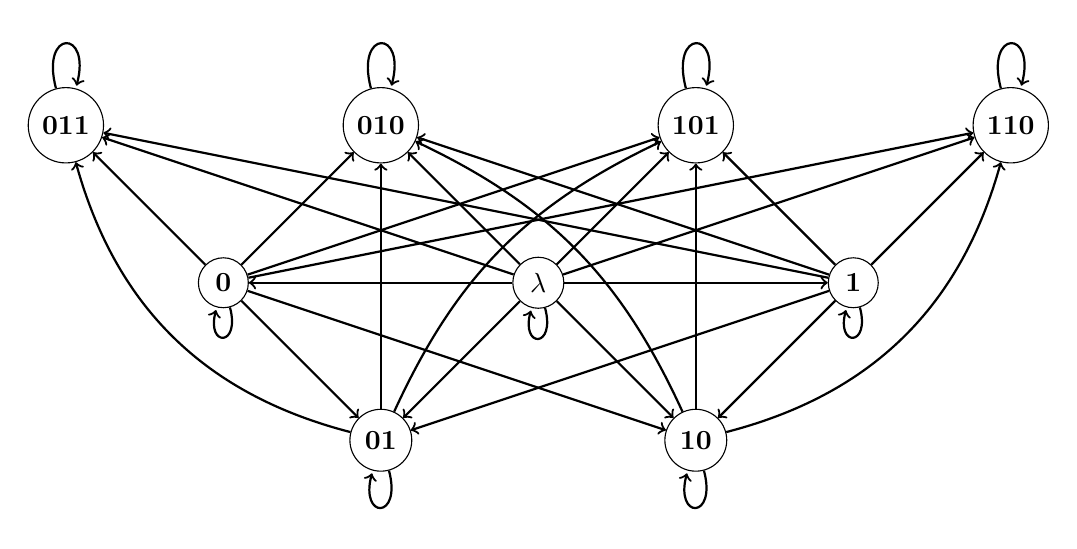
\begin{tikzpicture}
	
	\node[shape=circle,draw=black] (empty) at (6, 2)     {\textbf{$\lambda$}};
	\node[shape=circle,draw=black] (0) at (2, 2)     {\textbf{0}};
	\node[shape=circle,draw=black] (1) at (10, 2)     {\textbf{1}};
	\node[shape=circle,draw=black] (01) at (4, 0)     {\textbf{01}};
	\node[shape=circle,draw=black] (10) at (8, 0)     {\textbf{10}};
	\node[shape=circle,draw=black] (011) at (0, 4)     {\textbf{011}};
	\node[shape=circle,draw=black] (010) at (4, 4)     {\textbf{010}};
	\node[shape=circle,draw=black] (101) at (8, 4)     {\textbf{101}};
	\node[shape=circle,draw=black] (110) at (12, 4)     {\textbf{110}};

	\path[->, thick] (empty) edge [loop below] (empty);
	\path[->, thick] (0) edge [loop below] (0);
	\path[->, thick] (1) edge [loop below] (1);
	\path[->, thick] (01) edge [loop below] (01);
	\path[->, thick] (10) edge [loop below] (10);
	\path[->, thick] (010) edge [loop above] (101);
	\path[->, thick] (011) edge [loop above] (011);
	\path[->, thick] (101) edge [loop above] (101);
	\path[->, thick] (110) edge [loop above] (110);
	
	\path[->, thick] (empty) edge (0);
	\path[->, thick] (empty) edge (1);
	\path[->, thick] (empty) edge (01);
	\path[->, thick] (empty) edge (10);
	\path[->, thick] (empty) edge (010);
	\path[->, thick] (empty) edge (011);
	\path[->, thick] (empty) edge (101);
	\path[->, thick] (empty) edge (110);
	
	\path[->, thick] (0) edge (01);
	\path[->, thick] (0) edge (10);
	\path[->, thick] (0) edge (010);
	\path[->, thick] (0) edge (011);
	\path[->, thick] (0) edge (101);
	\path[->, thick] (0) edge (110);
	
	\path[->, thick] (1) edge (01);
	\path[->, thick] (1) edge (10);
	\path[->, thick] (1) edge (010);
	\path[->, thick] (1) edge (011);
	\path[->, thick] (1) edge (101);
	\path[->, thick] (1) edge (110);
	
	\path[->, thick] (01) edge [bend left=30] (011);
	\path[->, thick] (01) edge (010);
	\path[->, thick] (01) edge [bend left=20] (101);
	
	\path[->, thick] (10) edge [bend right=20] (010);
	\path[->, thick] (10) edge (101);
	\path[->, thick] (10) edge [bend right=30] (110);
	
	\end{tikzpicture} 
	\caption{Directed graph of R}	
	\label{g1}
\end{figure}
\subsection*{b}
A relation is called a partial order if it is reflexive, anti-symmetric, and transitive. So showing these three properties hold for $R$ will be enough to say it is an equivalence relation.\\
Let all $w_0, w_1, w_2 \in S$.
\begin{center}
    Every binary string is a substring of itself. $R$ is reflexive.\\
    \bigskip
    If $w_0$ is a substring of $w_1$ and $w_1$ is a substring of $w_0$ then $w_0 = w_1$. $R$ is anti-symmetric.\\
    \bigskip
    Whenever $w_0$ is a substring of $w_1$ and $w_1$ is a substring of $w_2$ then $w_0$ is a substring of $w_2$. $R$ is transitive.
\end{center}
\subsection*{c}
No, $(S, R)$ is not a total order. To prove it, a counter example can be constructed as elements $\{01, 110\}$ of $S$ are not comparable.
\subsection*{d}
\begin{figure}[H]
	\centering
	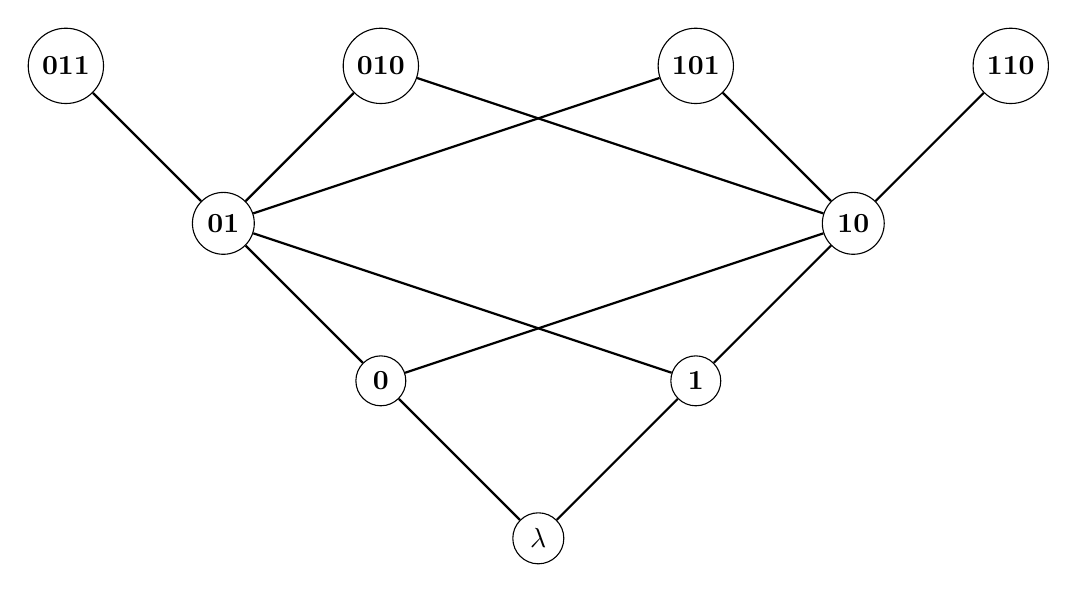
\begin{tikzpicture}
	
	\node[shape=circle,draw=black] (empty) at (6, 0)     {\textbf{$\lambda$}};
	\node[shape=circle,draw=black] (0) at (4, 2)     {\textbf{0}};
	\node[shape=circle,draw=black] (1) at (8, 2)     {\textbf{1}};
	\node[shape=circle,draw=black] (01) at (2, 4)     {\textbf{01}};
	\node[shape=circle,draw=black] (10) at (10, 4)     {\textbf{10}};
	\node[shape=circle,draw=black] (011) at (0, 6)     {\textbf{011}};
	\node[shape=circle,draw=black] (010) at (4, 6)     {\textbf{010}};
	\node[shape=circle,draw=black] (101) at (8, 6)     {\textbf{101}};
	\node[shape=circle,draw=black] (110) at (12, 6)     {\textbf{110}};
	
	\path[-, thick] (empty) edge (0);
	\path[-, thick] (empty) edge (1);
	
	\path[-, thick] (0) edge (01);
	\path[-, thick] (0) edge (10);
	
	\path[-, thick] (1) edge (01);
	\path[-, thick] (1) edge (10);
	
	\path[-, thick] (01) edge (011);
	\path[-, thick] (01) edge (010);
	\path[-, thick] (01) edge (101);
	
	\path[-, thick] (10) edge (010);
	\path[-, thick] (10) edge (101);
	\path[-, thick] (10) edge (110);
	
	\end{tikzpicture} 
	\caption{Hasse diagram of R}	
	\label{h1}
\end{figure}
Maximal elements are 011, 010, 101, 110.\\
Minimal element is $\lambda$.
\subsection*{e}
$(S, R)$ does not constitute a lattice. For example $011$ and $010$ does not have any least upper bound.

\section*{Answer 2}
\subsection*{a}
    \begin{table}[H]
    \centering
    \begin{tabular}{|l|l|}
    \hline
    \textbf{Vertex} & \textbf{Adjacent Vertices} \\ \hline
    a                                & a, b, d                                     \\
    b                                & d, c                                        \\
    c                                & b                                           \\
    d                                & c                                           \\
    e                                & b, f                                        \\
    f                                & b, e, f                                     \\
    g                                & c, f                                        \\ \hline
    \end{tabular}
    \end{table}
\subsection*{b}
Adjacency matrix with respect to the ordering of vertices a, b, c, d, e, f, g.
\[
  \begin{bmatrix}
    1 & 1 & 0 & 1 & 0 & 0 & 0 \\
    0 & 0 & 1 & 1 & 0 & 0 & 0 \\
    0 & 1 & 0 & 0 & 0 & 0 & 0 \\
    0 & 0 & 1 & 0 & 0 & 0 & 0 \\
    0 & 1 & 0 & 0 & 0 & 1 & 0 \\
    0 & 1 & 0 & 0 & 1 & 1 & 0 \\
    0 & 0 & 1 & 0 & 0 & 1 & 0 \\
  \end{bmatrix}
\]
\subsection*{c}
\begin{table}[H]
    \centering
    \begin{tabular}{|l|l|l|}
    \hline
    \textbf{Vertex} & \textbf{Indegree} & \textbf{Outdegree} \\ \hline
    a                                & 1                                  & 3                                   \\
    b                                & 4                                  & 2                                   \\
    c                                & 3                                  & 1                                   \\
    d                                & 2                                  & 1                                   \\
    e                                & 1                                  & 2                                   \\
    f                                & 3                                  & 3                                   \\
    g                                & 0                                  & 2                                   \\ \hline
    \end{tabular}
\end{table}
\subsection*{d}
\begin{table}[H]
    \centering
    \begin{tabular}{ll}
    a, a, b, d, c & f, e, b, d, c \\
    g, f, e, b, d & g, f, b, d, c \\
    f, f, b, d, c & f, f, e, b, d
    \end{tabular}
\end{table}
\subsection*{e}
\begin{table}[H]
    \centering
    \begin{tabular}{ll}
    e, f, f, e & b, d, c, b \\
    f, e, f, f & c, b, d, c \\
    f, f, e, f & d, c, b, d
    \end{tabular}
\end{table}
\subsection*{f}
G is not strongly connected since for example there is no path that reaches to g. But it is weakly connected because there is a path between every two vertices in the underlying undirected graph.
\subsection*{g}
Strongly-connected components of G are:
\begin{figure}[H]
	\centering
	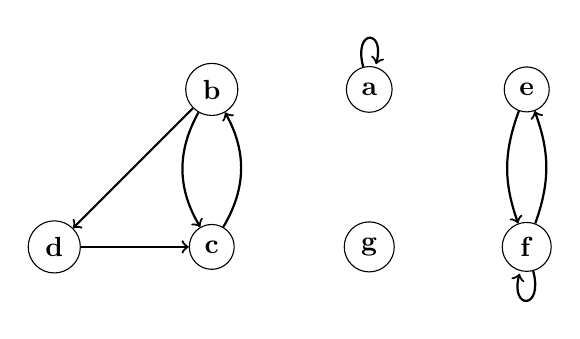
\begin{tikzpicture}
	
	\node[shape=circle,draw=black] (a) at (4, 2)     {\textbf{a}};
	\node[shape=circle,draw=black] (b) at (2, 2)     {\textbf{b}};
	\node[shape=circle,draw=black] (c) at (2, 0)     {\textbf{c}};
	\node[shape=circle,draw=black] (d) at (0, 0)     {\textbf{d}};
	\node[shape=circle,draw=black] (e) at (6, 2)     {\textbf{e}};
	\node[shape=circle,draw=black] (f) at (6, 0)     {\textbf{f}};
	\node[shape=circle,draw=black] (g) at (4, 0)     {\textbf{g}};

	\path[->, thick] (a) edge [loop above] (a);

	\path[->, thick] (b) edge (d);
	\path[->, thick] (b) edge [bend right=30] (c);
	\path[->, thick] (c) edge [bend right=30] (b);
	\path[->, thick] (d) edge (c);

	\path[->, thick] (e) edge [bend right=20] (f);
	\path[->, thick] (f) edge [bend right=20] (e);
	\path[->, thick] (f) edge [loop below] (f);

	\end{tikzpicture}	
	\label{g2}
\end{figure}
\subsection*{h}
\begin{table}[H]
    \centering
    \begin{tabular}{l}
    a, d, c, b \\
    a, b, d, c \\
    b, d, c, b \\
    c, b, d, c \\
    d, c, b, d
    \end{tabular}
\end{table}

\section*{Answer 3}
\subsection*{a}
Since it has an Euler circuit, as proved in part b, it also has an Euler path.
\subsection*{b}
Since it has more than 2 vertices and all of its vertices have even degrees(2, 6, 4, 4, 6, 6, 4, 4, 4, 6, 2 alphabetically), it has an Euler circuit.
\subsection*{c}
To talk about a Hamiltonian path we should consider the simple paths. So, we can use the below simplified version of G. We can see by observing that there is a Hamiltonian path as a, b, e, f, h, i, c, d, g, k, j.
\subsection*{d}
It does not have a Hamiltonian circuit. We can see from the below simplified version of G that there is only one vertex that connects right subgraph to the left one so in order to have a circuit we have to pass from c two times, therefore it can not have a Hamiltonian circuit.
\begin{figure}[H]
	\centering
	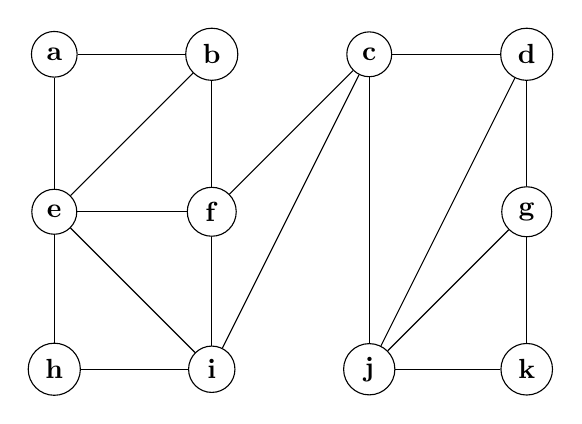
\begin{tikzpicture}[every loop/.style={}]
	
	\node[shape=circle,draw=black] (a) at (0, 4)     {\textbf{a}};
	\node[shape=circle,draw=black] (b) at (2, 4)     {\textbf{b}};
	\node[shape=circle,draw=black] (c) at (4, 4)     {\textbf{c}};
	\node[shape=circle,draw=black] (d) at (6, 4)     {\textbf{d}};
	\node[shape=circle,draw=black] (e) at (0, 2)     {\textbf{e}};
	\node[shape=circle,draw=black] (f) at (2, 2)     {\textbf{f}};
	\node[shape=circle,draw=black] (g) at (6, 2)     {\textbf{g}};
	\node[shape=circle,draw=black] (h) at (0, 0)     {\textbf{h}};
	\node[shape=circle,draw=black] (i) at (2, 0)     {\textbf{i}};
	\node[shape=circle,draw=black] (j) at (4, 0)     {\textbf{j}};
	\node[shape=circle,draw=black] (k) at (6, 0)     {\textbf{k}};
	

	\path[-] (a) edge (b);
	\path[-] (a) edge (e);
	\path[-] (b) edge (e);
	\path[-] (b) edge (f);
	\path[-] (c) edge (f);
	\path[-] (c) edge (i);
	\path[-] (c) edge (j);
	\path[-] (c) edge (d);
	\path[-] (d) edge (j);
	\path[-] (d) edge (g);
	\path[-] (e) edge (f);
	\path[-] (e) edge (h);
	\path[-] (e) edge (i);
	\path[-] (f) edge (i);
	\path[-] (g) edge (j);
	\path[-] (g) edge (k);
	\path[-] (h) edge (i);
	\path[-] (j) edge (k);
	\end{tikzpicture} 
	\caption{Simplified graph G.}
	\label{g3}
\end{figure}

\section*{Answer 4}
\subsection*{a}
It has $m+n$ vertices and $mn$ edges.
\subsection*{b}
If one of the disjoint sets have higher elements in it, since we have to alternately visit one node from each set, there won't be enough to complete the circuit. So one being odd and other even, they are not equal. It does not have a Hamiltonian circuit.

\newpage

\newcommand\encircle[1]{%
  \tikz[baseline=(X.base)] 
    \node (X) [draw, shape=circle, inner sep=0] {\strut #1};}

\section*{Answer 5}
\subsection*{a}
\begin{table}[H]
    \centering
    \begin{tabular}{l|lllllll|l}
    \begin{tabular}[c]{@{}l@{}}Current\\ Vertex\end{tabular} & u & v & w & x  & y  & z  & t  & \begin{tabular}[c]{@{}l@{}}Selected\\ Vertex\end{tabular} \\ \hline
    s                                                        & 4 & 5 & \encircle{3} &  $\infty$  &  $\infty$  & $\infty$ &  $\infty$  & w                                                         \\
    w                                                        & \encircle{4} & 5 & \encircle{3} & 11 &  $\infty$  & 15 &  $\infty$  & u                                                         \\
    u                                                        & \encircle{4} & \encircle{5} & \encircle{3} & 11 & 15 & 15 &  $\infty$  & v                                                         \\
    v                                                        & \encircle{4} & \encircle{5} & \encircle{3} & \encircle{7}  & 11 & 15 &  $\infty$  & x                                                         \\
    x                                                        & \encircle{4} & \encircle{5} & \encircle{3} & \encircle{7}  & \encircle{8}  & 13 &  $\infty$  & y                                                         \\
    y                                                        & \encircle{4} & \encircle{5} & \encircle{3} & \encircle{7}  & \encircle{8}  & \encircle{12} & 17 & z                                                         \\
    z                                                        & \encircle{4} & \encircle{5} & \encircle{3} & \encircle{7}  & \encircle{8}  & \encircle{12} & \encircle{15} & t                                                        
    \end{tabular}
\end{table}
It is 15.
\subsection*{b}
\begin{table}[h]
    \centering
    \begin{tabular}{ll}
    \textbf{Edge}   & \textbf{Weight} \\
    (x, y) & 1      \\
    (x, v) & 2      \\
    (v, w) & 3      \\
    (w, u) & 1      \\
    (w, s) & 3      \\
    (y, z) & 4      \\
    (z, t) & 3      \\
    \textbf{Total:} & 17
    \end{tabular}
\end{table}
\subsection*{c}
\begin{figure}[H]
	\centering
	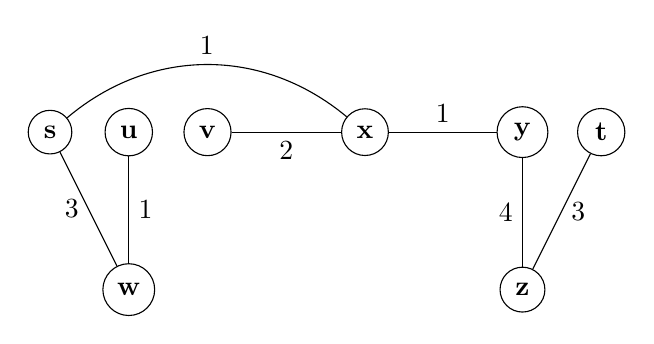
\begin{tikzpicture}
	\node[shape=circle,draw=black] (s) at (1, 2)     {\textbf{s}};
	\node[shape=circle,draw=black] (u) at (2, 2)     {\textbf{u}};
	\node[shape=circle,draw=black] (v) at (3, 2)     {\textbf{v}};
	\node[shape=circle,draw=black] (w) at (2, 0)     {\textbf{w}};
	\node[shape=circle,draw=black] (x) at (5, 2)     {\textbf{x}};
	\node[shape=circle,draw=black] (y) at (7, 2)     {\textbf{y}};
	\node[shape=circle,draw=black] (z) at (7, 0)     {\textbf{z}};
	\node[shape=circle,draw=black] (t) at (8, 2)     {\textbf{t}};

	\path[-] (u) edge node[right]{1} (w);
	\path[-] (v) edge node[below]{2} (x);
	\path[-] (w) edge node[left]{3} (s);
	\path[-] (x) edge [bend right=40] node[above]{1} (s);
	\path[-] (x) edge node[above]{1} (y);
	\path[-] (y) edge node[left]{4} (z);
	\path[-] (z) edge node[right]{3} (t);
		
	\end{tikzpicture}
	\caption{Add $(s, x, 1)$.}
	\label{5g1}
\end{figure}
\begin{figure}[H]
	\centering
	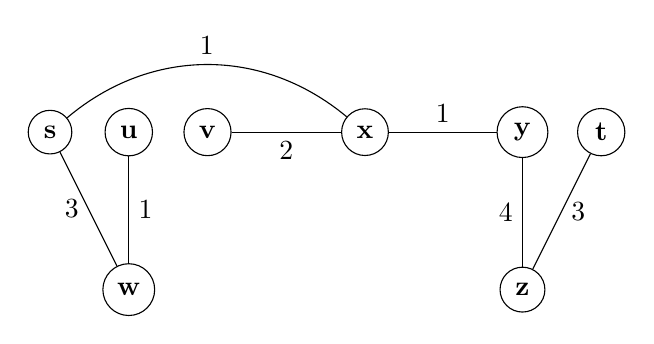
\begin{tikzpicture}
	\node[shape=circle,draw=black] (s) at (1, 2)     {\textbf{s}};
	\node[shape=circle,draw=black] (u) at (2, 2)     {\textbf{u}};
	\node[shape=circle,draw=black] (v) at (3, 2)     {\textbf{v}};
	\node[shape=circle,draw=black] (w) at (2, 0)     {\textbf{w}};
	\node[shape=circle,draw=black] (x) at (5, 2)     {\textbf{x}};
	\node[shape=circle,draw=black] (y) at (7, 2)     {\textbf{y}};
	\node[shape=circle,draw=black] (z) at (7, 0)     {\textbf{z}};
	\node[shape=circle,draw=black] (t) at (8, 2)     {\textbf{t}};

	\path[-] (u) edge node[right]{1} (w);
	\path[-] (v) edge node[below]{2} (x);
	\path[-] (w) edge node[left]{3} (s);
	\path[-] (x) edge [bend right=40] node[above]{1} (s);
	\path[-] (x) edge node[above]{1} (y);
	\path[-] (y) edge node[left]{4} (z);
	\path[-] (z) edge node[right]{3} (t);
		
	\end{tikzpicture}
	\caption{Add $(t, u, 6)$.}
	\label{5g2}
\end{figure}
\begin{figure}[H]
	\centering
	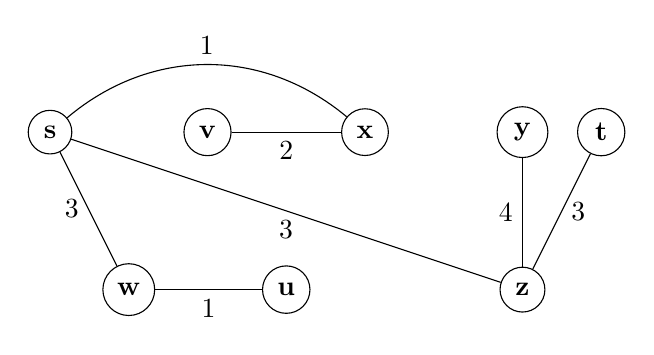
\begin{tikzpicture}
	\node[shape=circle,draw=black] (s) at (1, 2)     {\textbf{s}};
	\node[shape=circle,draw=black] (u) at (4, 0)     {\textbf{u}};
	\node[shape=circle,draw=black] (v) at (3, 2)     {\textbf{v}};
	\node[shape=circle,draw=black] (w) at (2, 0)     {\textbf{w}};
	\node[shape=circle,draw=black] (x) at (5, 2)     {\textbf{x}};
	\node[shape=circle,draw=black] (y) at (7, 2)     {\textbf{y}};
	\node[shape=circle,draw=black] (z) at (7, 0)     {\textbf{z}};
	\node[shape=circle,draw=black] (t) at (8, 2)     {\textbf{t}};

	\path[-] (u) edge node[below]{1} (w);
	\path[-] (v) edge node[below]{2} (x);
	\path[-] (w) edge node[left]{3} (s);
	\path[-] (x) edge [bend right=40] node[above]{1} (s);
	\path[-] (y) edge node[left]{4} (z);
	\path[-] (z) edge node[right]{3} (t);
	\path[-] (s) edge node[below]{3} (z);
		
	\end{tikzpicture}
	\caption{Add $(s, z, -3)$.}
	\label{5g3}
\end{figure}
\begin{figure}[H]
	\centering
	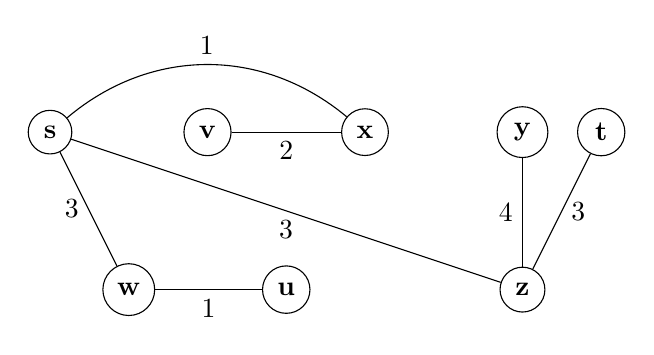
\begin{tikzpicture}
	\node[shape=circle,draw=black] (s) at (1, 2)     {\textbf{s}};
	\node[shape=circle,draw=black] (u) at (4, 0)     {\textbf{u}};
	\node[shape=circle,draw=black] (v) at (3, 2)     {\textbf{v}};
	\node[shape=circle,draw=black] (w) at (2, 0)     {\textbf{w}};
	\node[shape=circle,draw=black] (x) at (5, 2)     {\textbf{x}};
	\node[shape=circle,draw=black] (y) at (7, 2)     {\textbf{y}};
	\node[shape=circle,draw=black] (z) at (7, 0)     {\textbf{z}};
	\node[shape=circle,draw=black] (t) at (8, 2)     {\textbf{t}};

	\path[-] (u) edge node[below]{1} (w);
	\path[-] (v) edge node[below]{2} (x);
	\path[-] (w) edge node[left]{3} (s);
	\path[-] (x) edge [bend right=40] node[above]{1} (s);
	\path[-] (y) edge node[left]{4} (z);
	\path[-] (z) edge node[right]{3} (t);
	\path[-] (s) edge node[below]{3} (z);
		
	\end{tikzpicture}
	\caption{Add $(u, y, 3)$.}
	\label{5g4}
\end{figure}
\begin{figure}[H]
	\centering
	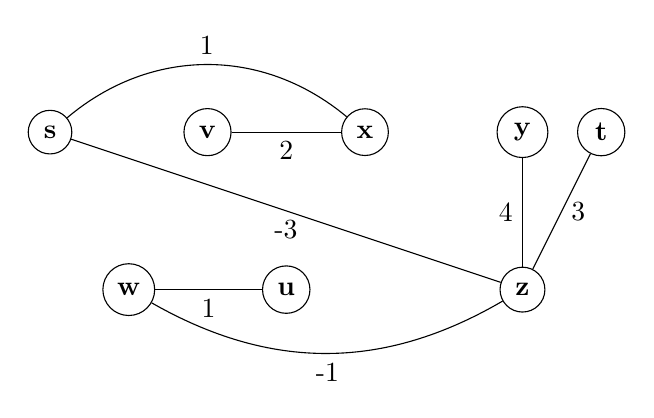
\begin{tikzpicture}
	\node[shape=circle,draw=black] (s) at (1, 2)     {\textbf{s}};
	\node[shape=circle,draw=black] (u) at (4, 0)     {\textbf{u}};
	\node[shape=circle,draw=black] (v) at (3, 2)     {\textbf{v}};
	\node[shape=circle,draw=black] (w) at (2, 0)     {\textbf{w}};
	\node[shape=circle,draw=black] (x) at (5, 2)     {\textbf{x}};
	\node[shape=circle,draw=black] (y) at (7, 2)     {\textbf{y}};
	\node[shape=circle,draw=black] (z) at (7, 0)     {\textbf{z}};
	\node[shape=circle,draw=black] (t) at (8, 2)     {\textbf{t}};

	\path[-] (u) edge node[below]{1} (w);
	\path[-] (v) edge node[below]{2} (x);
	\path[-] (x) edge [bend right=40] node[above]{1} (s);
	\path[-] (y) edge node[left]{4} (z);
	\path[-] (z) edge node[right]{3} (t);
	\path[-] (s) edge node[below]{-3} (z);
	\path[-] (w) edge [bend right=30] node[below]{-1} (z);
		
	\end{tikzpicture}
	\caption{Add $(w, z, -1)$.}
	\label{5g5}
\end{figure}
\subsection*{d}
Yes we can.
\newpage

\section*{Answer 6}
\subsection*{a}
T has 13 vertices, 12 edges and the height of 4.
\subsection*{b}
33, 26, 35, 37, 34, 41, 61, 71, 63, 99, 98, 75, 42.
\subsection*{c}
26, 33, 34, 35, 37, 42, 41, 63, 61, 71, 75, 98, 99.
\subsection*{d}
42, 34, 26, 33, 37, 35, 75, 63, 41, 71, 61, 98, 99.
\subsection*{e}
No it is not. The nodes 26, 37, 71, 98 has only one child.
\subsection*{f}
No it is not. The nodes 41, 61 are not in the place that they should be with respect to the $\leq$ relation.
\subsection*{g}
Since in every height we can proceed only with one leaf, it is $3h+1$.
\subsection*{h}
\begin{figure}[H]
	\centering
	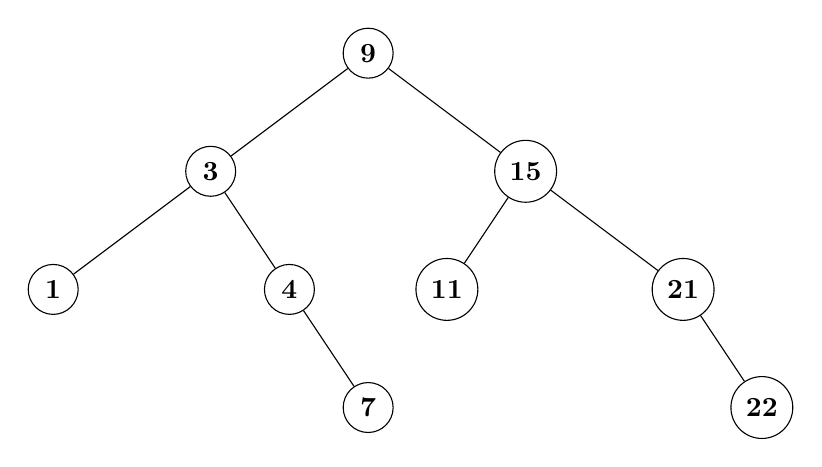
\begin{tikzpicture}
	
	\node[shape=circle,draw=black] (p) at (7, 4.5)     {\textbf{9}};
	\node[shape=circle,draw=black] (q) at (5, 3)     {\textbf{3}};
	\node[shape=circle,draw=black] (r) at (9, 3)     {\textbf{15}};
	\node[shape=circle,draw=black] (s) at (3, 1.5)     {\textbf{1}};
	\node[shape=circle,draw=black] (t) at (6, 1.5)     {\textbf{4}};
	\node[shape=circle,draw=black] (u) at (8, 1.5)    {\textbf{11}};
	\node[shape=circle,draw=black] (v) at (11, 1.5)     {\textbf{21}};
	\node[shape=circle,draw=black] (x) at (12, 0)     {\textbf{22}};
	\node[shape=circle,draw=black] (y) at (7, 0)     {\textbf{7}};
		
	\path[-] (p) edge (q);
	\path[-] (p) edge (r);
	\path[-] (q) edge (t);
	\path[-] (q) edge (s);
	\path[-] (r) edge (u);
	\path[-] (r) edge (v);
	\path[-] (v) edge (x);
	\path[-] (t) edge (y);
	\end{tikzpicture} 
	\caption{Binary Search Tree for Q6.h.}	
	\label{binshtree}
\end{figure}
\subsection*{i}
For key value 2: 9, 3, 1\\
For key value 22: 9, 15, 21, 22
\subsection*{j}
\begin{figure}[H]
	\centering
	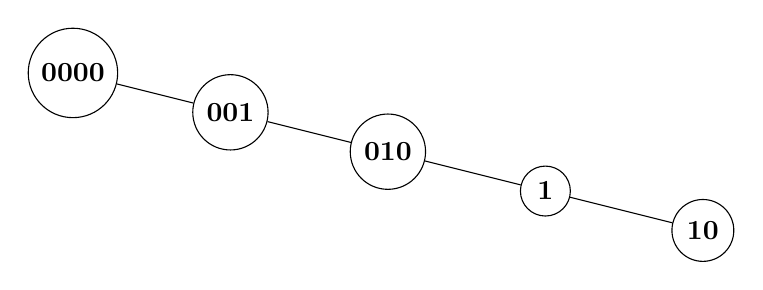
\begin{tikzpicture}
	
	\node[shape=circle,draw=black] (p) at (0, 2)     {\textbf{0000}};
	\node[shape=circle,draw=black] (q) at (2, 1.5)     {\textbf{001}};
	\node[shape=circle,draw=black] (r) at (4, 1)     {\textbf{010}};
	\node[shape=circle,draw=black] (s) at (6, 0.5)     {\textbf{1}};
	\node[shape=circle,draw=black] (t) at (8, 0)     {\textbf{10}};
	
	\path[-] (p) edge (q);
	\path[-] (q) edge (r);
	\path[-] (r) edge (s);
	\path[-] (s) edge (t);
	\end{tikzpicture} 
	\caption{Binary Search Tree for Q6.j.}	
	\label{binsjtree}
\end{figure}
\subsection*{k}
For key value 001: 0000, 001\\
For key value 011: 0000, 001, 010, 1
\subsection*{l}

\end{document}

​

